%!TEX program = xelatex
\documentclass{beamer}

\usepackage[citestyle=authoryear]{biblatex}
\addbibresource{./references.bib}
\usepackage{amsmath}
\usepackage{textpos}
\usepackage{blindtext}
\usepackage{graphicx}
\graphicspath{{./figs/}}
\usepackage{hyperref}

\usetheme{Imperial}

\title{A numerical investigation of hydrocarbon related magnetic signatures}
%\subtitle{}
\author{Miguel A. Valdez G.}
\email{mav113@ic.ac.uk}
\institute{Dept. Earth Sci. Eng. Imperial College London}
\date{15 February, 2018}
\event{\textit{Viva Voce} examination}

\setcounter{showSlideNumbers}{1}

\begin{document}
	\setcounter{showProgressBar}{0}
	\setcounter{showSlideNumbers}{0}

        \begin{frame}
          \titlepage
          \begin{tikzpicture}[remember picture,overlay]
            \node[anchor=north west] at (current page.north west) {
\includegraphics[height=0.8cm]{imperial_logo.eps}};
          \end{tikzpicture}
          \begin{tikzpicture}[remember picture,overlay]
            \useasboundingbox (0,0) rectangle(\the\paperwidth,\the\paperheight);
            \node[anchor=south] at (0.2\slidewidth,-4) {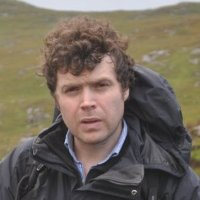
\includegraphics[height=0.15\slideheight]{adrianmux.jpg}};
            \node[anchor=north] at (0.2\slidewidth,-4) {\color{ImperialNavy}Adrian R. Muxworthy};
            \node[anchor=north] at (0.2\slidewidth,-4.4) {\color{ImperialBlue}\textit{ESE Imperial College}};
            \node[anchor=south] at (0.65\slidewidth,-4) {
\includegraphics[height=0.15\slideheight]{wynwilliams.jpg}};
            \node[anchor=north] at (0.65\slidewidth,-4) {\color{ImperialNavy}Wyn Williams};
            \node[anchor=north] at (0.65\slidewidth,-4.4) {\color{ImperialBlue}\textit{S. GeoSc. U. Edinburgh}};
          \end{tikzpicture}
        \end{frame}

        \addtobeamertemplate{frametitle}{}{%
          \begin{tikzpicture}[remember picture,overlay]
            \node[anchor=north east,yshift=2pt] at (current page.north east) {
\includegraphics[height=0.8cm]{imperial_logo.eps}};
          \end{tikzpicture}
        }

	\setcounter{framenumber}{0}
	\setcounter{showProgressBar}{1}
	\setcounter{showSlideNumbers}{1}

	\section{Introduction}

        \tikzset{
          mynode/.style={
            anchor=north west,
            align=left,
            text width=\slidewidth-1cm,
            execute at begin node=\setlength{\baselineskip}{0.25cm}
          }
        }

		\begin{frame}
			\frametitle{Why greigite?}
                        The thesis focuses on numerical simulations of the magnetic properties of greigite
			\begin{itemize}
%                        \item Iron sulphide analogue of magnetite
				\item Complex, unstable remanence carrier (usually authigenic in origin)
                                  \begin{itemize}
                                    \item Sediments$^{\text{1}}$
                                    \item Oil field overburdens$^{\text{2}}$
                                    \item Product of biomineralisation$^{\text{3}}$
                                  \end{itemize}
                                \item \textit{Few} numerical studies$^{\text{4}}$
				\item Magnetic parameters measurements fairly recent$^{\text{5,6,7}}$
			\end{itemize}
                  \begin{tikzpicture}[remember picture,overlay]
                    \useasboundingbox (0,0) rectangle(\the\paperwidth,\the\paperheight);
                    \draw [semithick,color=ImperialNavy] (0,0.35) -- (6,0.35);
                    \node[anchor=north west] at (0,0.35) {\color{ImperialNavy}\tiny{$^\text{1}$\textcite{Roberts2011}}};
                    \node[anchor=north west] at (0,0.1) {\color{ImperialNavy}\tiny{$^\text{2}$\textcite{Reynolds1993}}};
                    \node[anchor=north west] at (0,-0.15) {\color{ImperialNavy}\tiny{$^\text{3}$\textcite{Bazylinski1995}}};
                    \node[mynode] at (0,-0.4) {\color{ImperialNavy}\tiny{$^\text{4}$\textcite{Muxworthy2013}}};
                    \node[mynode] at (0,-0.65) {\color{ImperialNavy}\tiny{$^\text{5}$\textcite{Chang2008}}};
                    \node[mynode] at (0,-0.9) {\color{ImperialNavy}\tiny{$^\text{6}$\textcite{Winklhofer2014}}};
                    \node[mynode] at (0,-1.15) {\color{ImperialNavy}\tiny{$^\text{7}$\textcite{Li2014}}};
                  \end{tikzpicture}
		\end{frame}

%                \begin{frame}
%                  \frametitle{Magnetic parameters}
%                  \begin{itemize}
%                    \item Saturation magnetisation (from hysteresis data-fitting)$^\text{1}$: \\
%                          $\textit{M}_\text{S}=\text{3.51}\,\mu_\text{B}\,\, \text{p.c.u.}$
%                    \item Exchange stiffness constant (from Bloch spin-wave expansion)$^\text{2}$: \\
%                          $\textit{A}=\text{2}\times \text{10}^{\text{-12}}\, \text{J/m}$
%                    \item First MCA constant (from FMR powder spectra)$^\text{3}$: \\
%                          $\textit{K}_\text{1}=\text{-1.7}\times \text{10}^{\text{4}}\, \text{J/m}^\text{3}$
%%                    \item Curie temperature = \alert{?} (but most likely $>$250 C)
%                  \end{itemize}
%                  \begin{tikzpicture}[remember picture,overlay]
%                    \useasboundingbox (0,0) rectangle(\the\paperwidth,\the\paperheight);
%                    \draw [semithick,color=ImperialNavy] (0,0.35) -- (6,0.35);
%                    \node[anchor=north west] at (0,0.35) {\color{ImperialNavy}\tiny{$^\text{1}$\textcite{Guowei}}};
%                    \node[anchor=north west] at (0,0.1) {\color{ImperialNavy}\tiny{$^\text{2}$\textcite{Chang}}};
%                    \node[anchor=north west] at (0,-0.15) {\color{ImperialNavy}\tiny{$^\text{3}$\textcite{Winkl}}};
%                  \end{tikzpicture}
%                \end{frame}

                \begin{frame}
                  \frametitle{Previous studies}
                  \begin{itemize}
                    \item Analytical work$^\text{1}$
                      \begin{itemize}
                        \item cubes SD-PSD threshold $=$250 nm
                        \item \alert{parameters from poor samples or guessed}
                      \end{itemize}
                    \item Numerical work$^{\text{2}}$
                      \begin{itemize}
                        \item \alert{much better parameters!}
                        \item cubes SD-PSD threshold $=$60 nm
                        \item good agreement with prev. analytical work once new parameters accounted for
                        \item \alert{however...}
                          \begin{itemize}
                            \item only cuboidal shapes (FD model)
                            \item new $\textit{M}_{\text{S}}\sim\text{10}\text{\%}$ higher
                          \end{itemize}
                      \end{itemize}
                  \end{itemize}
                  \begin{tikzpicture}[remember picture,overlay]
                    \useasboundingbox (0,0) rectangle(\the\paperwidth,\the\paperheight);
                    \draw [semithick,color=ImperialNavy] (0,0.35) -- (6,0.35);
                    \node[mynode] at (0,0.35) {\color{ImperialNavy}\tiny{$^\text{1}$\textcite{Diaz-Ricci1992}}};
                    \node[mynode] at (0,0.1) {\color{ImperialNavy}\tiny{$^\text{2}$\textcite{Muxworthy2013}}};
                  \end{tikzpicture}
                \end{frame}
                
	\section{Methodology}
        
        \begin{frame}
          \frametitle{Micromagnetics}
          Aims to find the equilibrium magnetisation of a ferromagnet\\
          \color{ImperialNavy}\huge{Two approaches:}
               \begin{enumerate}
                 \item \color{ImperialBlue}\large{Energy minimisation (fast! but less robust...)}
                 \item \color{ImperialBlue}\large{Solve the LLG (slower...but more physical!)}\\
                   ...essentially torque minimisation
               \end{enumerate}
          \begin{columns}
            \begin{column}{0.5\textwidth}
              \color{black}{\large{En. min. for minimal action paths and FORC modelling:}}
              \begin{itemize}
                \item \textit{FEM-BEM} package \alert{MERRILL} from Edinburgh
              \end{itemize}
            \end{column}
            \begin{column}{0.5\textwidth}
              \color{black}{\large{LLG for domain state energy size/shape dependence:}}
              \begin{itemize}
                \item \textit{FEniCS} based parallelised FEM package \alert{DUNLOP} from Edinburgh
              \end{itemize}
            \end{column}
          \end{columns}
        \end{frame}


        \begin{frame}
          \frametitle{Micromagnetics}
          \color{ImperialNavy}\huge{The micromagnetic energy:}
          \begin{enumerate}
                  \item Given $\textbf{\textit{m}}$ ($|\textbf{\textit{m}}|^\text{2}=\text{1}$) find the energy:\\
                  \vspace{2mm}
                  \large $\textit{E}_{\text{G}}=\int_{\textit{V}}\phi_{\text{G}}\,\text{d}\textit{V}$\\
                  \vspace{2mm}
                  $\textit{E}_{\text{G}}=\int_{\textit{V}}\left(\phi_{\text{ex.}}+\phi_{\text{anis.}}+\phi_{\text{str.}}+\phi_{\text{ext.}}\right)\,\text{d}\textit{V}$\\
                  \vspace{2mm}
                  is the sum of exchange, anisotropy, stray field and external field energies$^{\text{1}}$\\
                  \vspace{4mm}
                  \begin{tikzpicture}[remember picture,overlay]
                    \useasboundingbox (0,0) rectangle(\the\paperwidth,\the\paperheight);
                    \draw [semithick,color=ImperialNavy] (0,0.35) -- (6,0.35);
                    \node[anchor=north west] at (0,0.35) {\color{ImperialNavy}\tiny{$^\text{1}$\textcite{Brown}}};
                  \end{tikzpicture}
          \end{enumerate}
        \end{frame}

        \begin{frame}
          \frametitle{Micromagnetics}
          \color{ImperialNavy}\huge{The exchange energy:}\\
          \center $\phi_{\text{ex.}}=\textit{A}|\nabla\textbf{\textit{m}}|^\text{2}$\\
          \flushleft \large \alert{favours uniform magnetisations}
        \end{frame}


        \begin{frame}
          \frametitle{Micromagnetics}
          \color{ImperialNavy}\huge{The magnetocrystalline anisotropy energy:}\\
          \Large  $\phi_{\text{anis.}}=(\textit{K}_\text{1}/\text{2})\sum_{\textit{i}\neq \textit{j}}\gamma_{\textit{i}}^{\text{2}}\gamma_{\textit{j}}^{\text{2}} + \textit{K}_{\text{2}}\prod_{\textit{i}}\gamma_{\textit{i}}^{\text{2}}$\\
                  $\phi_{\text{anis.}}=\textit{K}_\text{1}\left( \textit{m}_{\textit{x}}^{\text{2}}\textit{m}_{\textit{y}}^{\text{2}}+\textit{m}_{\textit{y}}^{\text{2}}\textit{m}_{\textit{z}}^{\text{2}}+\textit{m}_{\textit{z}}^{\text{2}}\textit{m}_{\textit{x}}^{\text{2}}  \right)$,  $\text{K}_\text{1}\gg\text{K}_\text{2}$\\
        \vspace{2mm} \large \alert{favours alignment with so-called easy axes}
        \end{frame}


        \begin{frame}
          \frametitle{Micromagnetics}
          \color{ImperialNavy}\huge{The stray field energy:}\\
          \center $\phi_{\text{str.}}=-\mu_{\text{0}}\textit{M}_{\text{S}}/\text{2}(\textbf{\textit{m}}\cdot\textbf{\textit{H}}_{\text{str.}})$\\
          \vspace{2mm} \flushleft \large \alert{favours flux closures}
        \end{frame}


        \begin{frame}
          \frametitle{Micromagnetics}
          \color{ImperialNavy}\huge{The external field energy:}\\
          \center $\phi_{\text{ext.}}=-\mu_{\text{0}}\textit{M}_{\text{S}}\textbf{\textit{m}}\cdot\textbf{\textit{H}}_{\text{ext.}}$
          \vspace{2mm} \flushleft \large \alert{favours alignment with external field}\\
          \vspace{4mm} \LARGE \alert{2.} Minimise! $\rightarrow$  $\delta\textit{E}_{\text{G}}/\delta\textbf{\textit{m}}=\text{0}$
        \end{frame}


        \begin{frame}
          \frametitle{Micromagnetics}
          \color{ImperialNavy}\huge{The LLG equation$^{\text{1}}$:}
          \begin{enumerate}
            \item Given $\textbf{\textit{m}}$ find the \alert{\textit{effective}} field\\
            $\textbf{\textit{H}}_{\text{eff.}}=-(\text{1}/\mu_{\text{0}}\textit{M}_{\text{S}})\partial\phi_{\text{G}}/\partial\textbf{\textit{m}}$
            \item Solve for $\textbf{\textit{m}}$\\
            $\partial\textbf{\textit{m}}/\partial\textit{t} = -\gamma^{'}\textbf{\textit{m}}\times\textbf{\textit{H}}_{\text{eff.}} - \alpha\gamma^{'}\textbf{\textit{m}}\times(\textbf{\textit{m}}\times\textbf{\textit{H}}_{\text{eff.}})$, \\
            \vspace{2mm} where $\alpha$ \alert{the damping constant} (usually 1 -- 10),\\
            $\gamma^{'}=\gamma/(\text{1}+\alpha^{\text{2}})$, and $\gamma$ \alert{the gyromagnetic ratio}
          \end{enumerate}
          \begin{tikzpicture}[remember picture,overlay]
            \useasboundingbox (0,0) rectangle(\the\paperwidth,\the\paperheight);
            \draw [semithick,color=ImperialNavy] (0,0.35) -- (6,0.35);
            \node[anchor=north west] at (0,0.35) {\color{ImperialNavy}\tiny{$^\text{1}$\textcite{Gilbert2004}}};
          \end{tikzpicture}
        \end{frame}

        \section{Research Chapter I}
        \begin{frame}
          \frametitle{Domain structures}
          First, to probe greigite's domain state dependence on size and shape
          \begin{itemize}
            \item \color{ImperialNavy}\textit{LLG }from \alert{30 nm to 300 nm}
            \item for a variety of \alert{shapes}
            \item \textit{FEniCS} based parallelised package \alert{DUNLOP} from Edinburgh
          \end{itemize}
          \color{ImperialProcessBlue}\Large{...but are they stable?}
        \end{frame}

        \begin{frame}
          \frametitle{Blocking volumes}
          The probability of a transition from one \textit{LEM} state to another tends to 1 as the observation time tends to $\tau=\tau_{\text{0}}\textit{e}^{\left(\textit{E}_{\textit{B}}/\textit{K}_{\text{B}}\textit{T}\right)}$, with
          \begin{itemize}
            \item $\textit{K}_{\text{B}}$ \alert{Boltzmann's constant}
            \item $\textit{T}$ \alert{the temperature}
            \item $\tau_{\text{0}}$ \alert{the attempt time} (usually 10$^{\text{-9}}$ s)
            \item $\textit{E}_{\textit{B}}$ \alert{the energy barrier} along an action-minimising path
          \end{itemize}
          Blocking volume is one at which the relaxation time surpasses \alert{four billion years} (10$^{\text{9}}$).
        \end{frame}

        \begin{frame}
          \frametitle{Blocking volumes}
          To estimate greigite's blocking volume
          \begin{itemize}
            \item at each size and shape \alert{obtain the LEMs}
            \item \color{ImperialNavy}calculate \alert{action-minimising paths} between GEMs
            \item \textit{FEM-BEM} package \alert{MERRILL} from Edinburgh
            \item for a variety of \alert{shapes}
            \item \alert{from 30 nm} until blocking volume is found

          \end{itemize}
        \end{frame}

		\begin{frame}
                  \frametitle{Nat. morphologies}
                  \begin{figure}[htb]
                    \centering
                    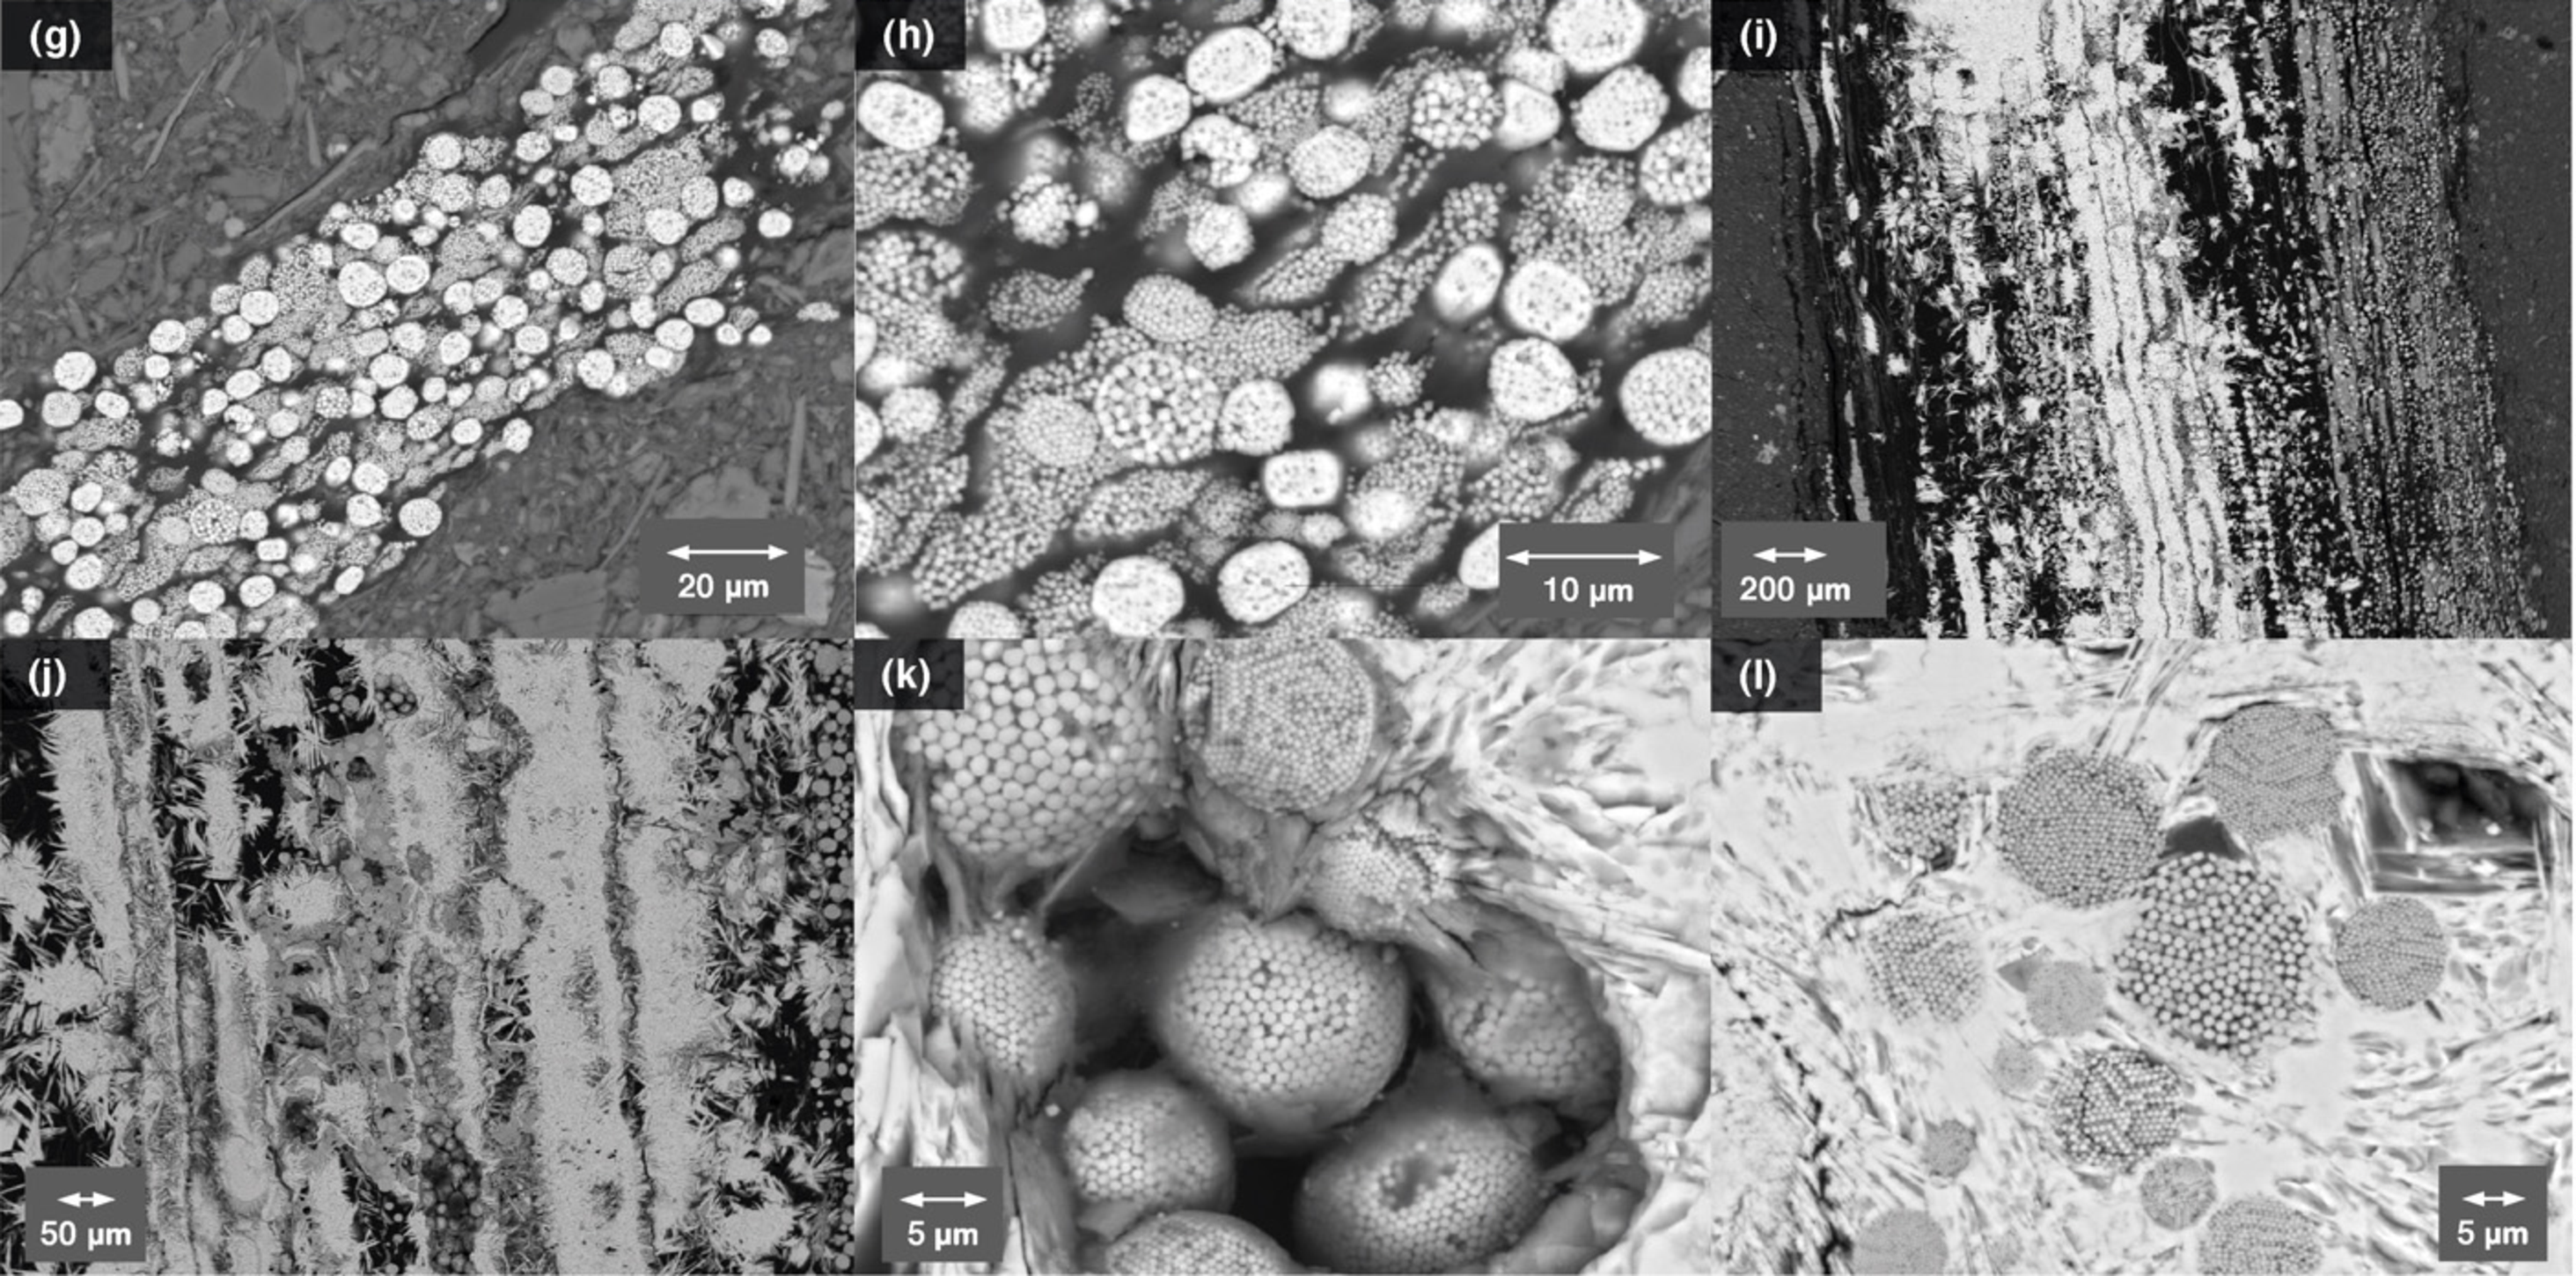
\includegraphics[width=\textwidth]{greigite_framboids.pdf}
                    \caption{SEM images of iron sulphide minerals (from \textcite{Roberts2015}, reproduced with permission from the author)}
                  \end{figure}
		\end{frame}

                \begin{frame}
                  \frametitle{Model morphologies}
                  \begin{figure}[htb]
                    \centering
                    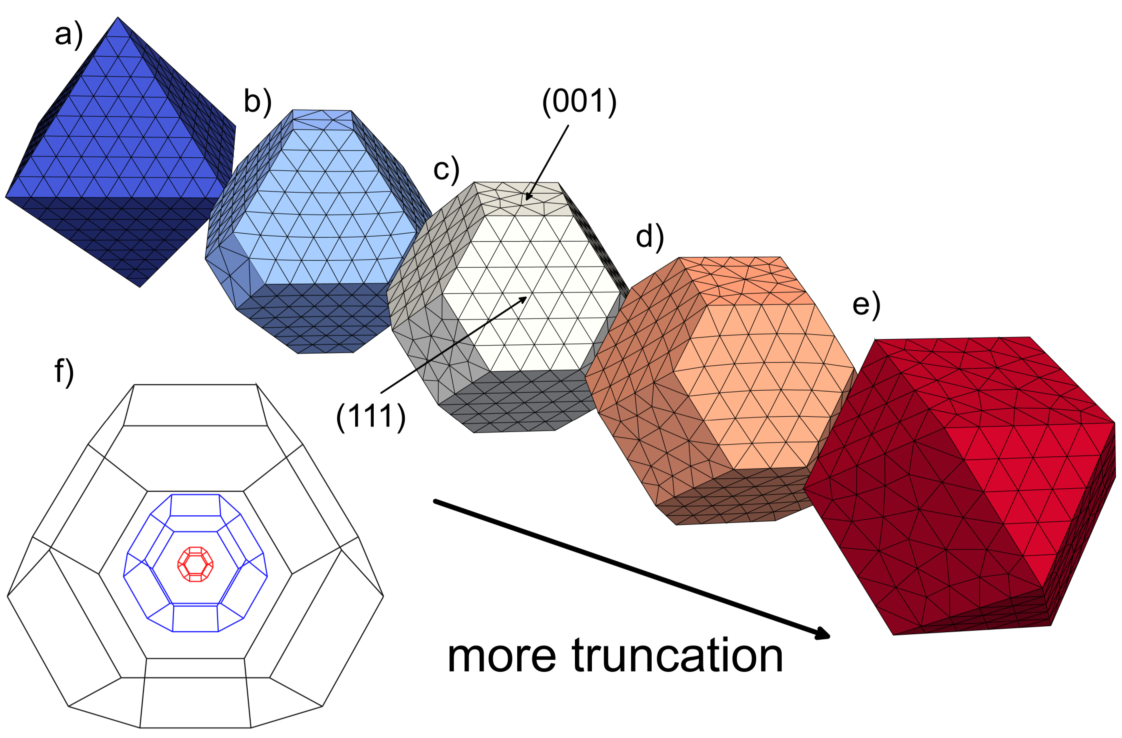
\includegraphics[width=0.9\textwidth]{Chapter_01_Figure_01.pdf}
%                    \caption{The model morphologies}
                  \end{figure}
                \end{frame}

                \begin{frame}
                  \frametitle{Crystal growth model}
                  \begin{figure}[htb]
                    \centering
                    \includegraphics[width=0.95\textwidth]{Chapter_01_spheres.pdf}
                  \end{figure}
                \end{frame}

                \begin{frame}
                  \frametitle{En. size/shape dependence}
                  \begin{figure}[htb]
                    \centering
                    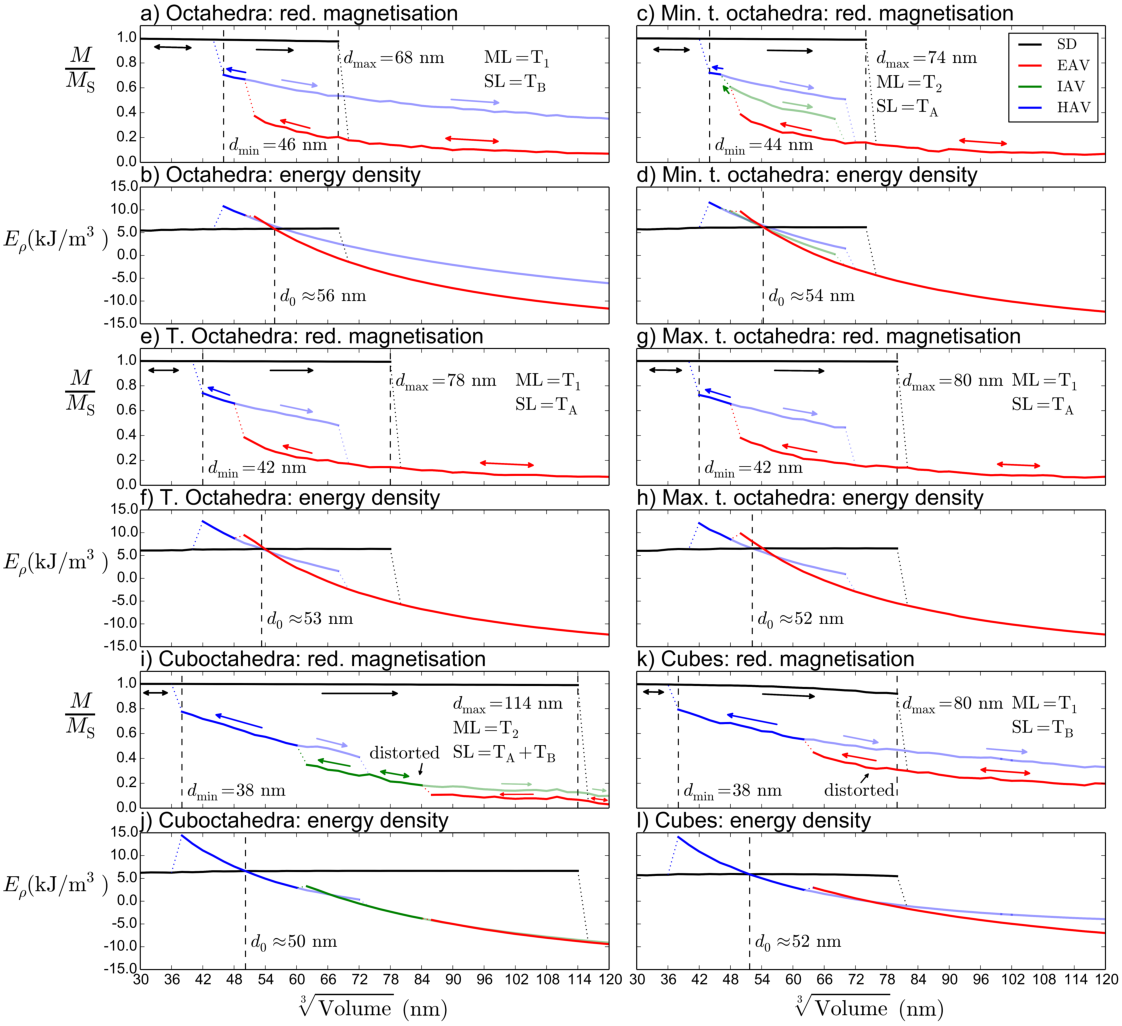
\includegraphics[width=0.8\textwidth]{Chapter_01_Figure_03.pdf}
                  \end{figure}
                \end{frame}

                \begin{frame}
                  \frametitle{Magnetic structures}
                  \begin{figure}[htb]
                    \centering
                    \includegraphics[width=0.9\textwidth]{Chapter_01_Figure_04.pdf}
                  \end{figure}
                \end{frame}

                \begin{frame}
                  \frametitle{Magnetic structures}
                  \begin{figure}[htb]
                    \centering
                    \includegraphics[width=0.9\textwidth]{Chapter_01_Figure_05.pdf}
                  \end{figure}
                \end{frame}

                \begin{frame}
                  \frametitle{SV to MD transition?}
                  \begin{figure}[htb]
                    \centering
                    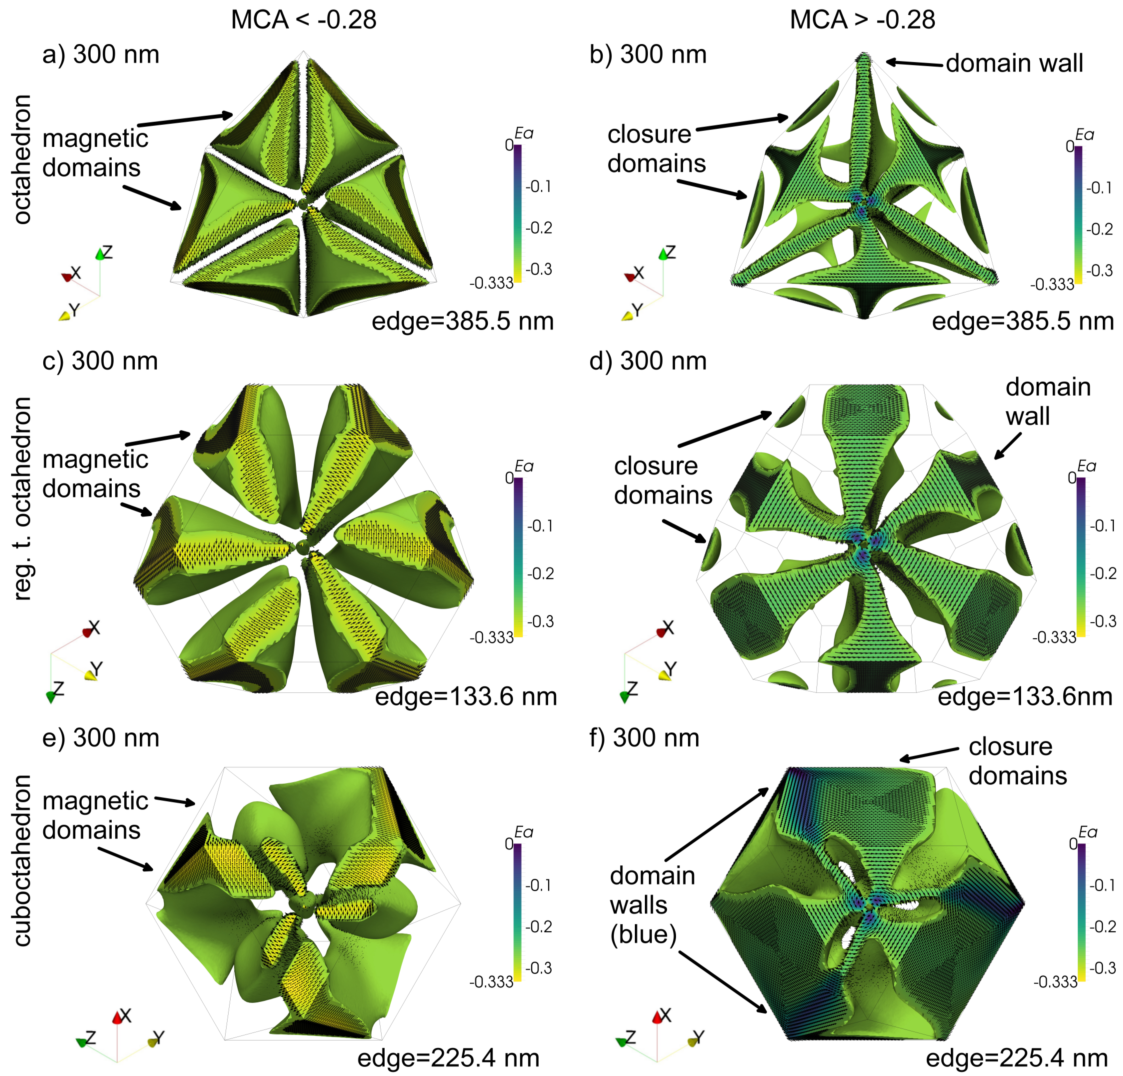
\includegraphics[width=0.7\textwidth]{Chapter_01_Figure_06.pdf}
                  \end{figure}
                \end{frame}


                \begin{frame}
                  \frametitle{Minimal action paths}
                  \begin{figure}[htb]
                    \centering
                    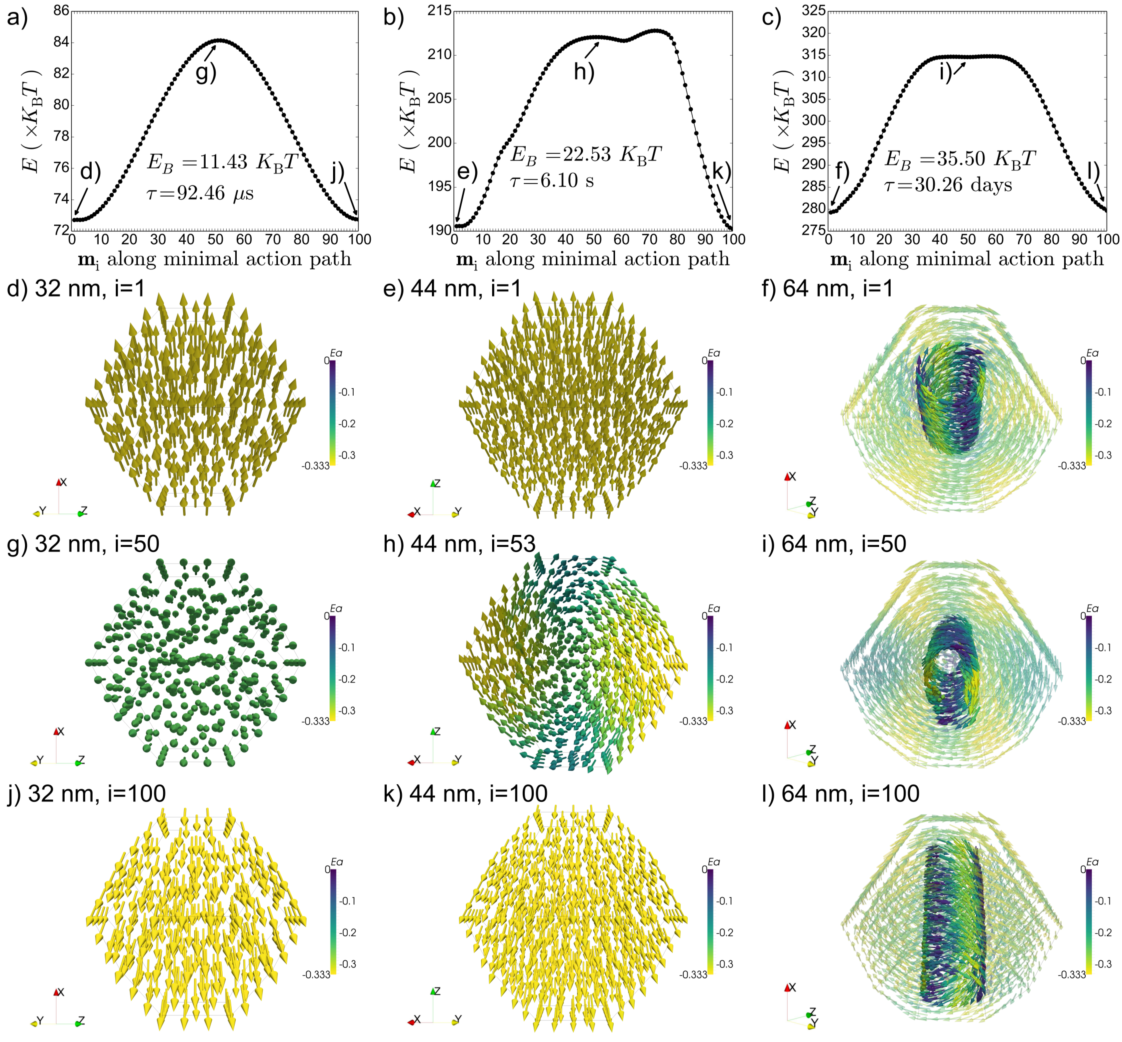
\includegraphics[width=0.76\textwidth]{Chapter_01_Figure_07.pdf}
                  \end{figure}
                \end{frame}


                \begin{frame}
                  \frametitle{Minimal action paths}
                  \begin{figure}[htb]
                    \centering
                    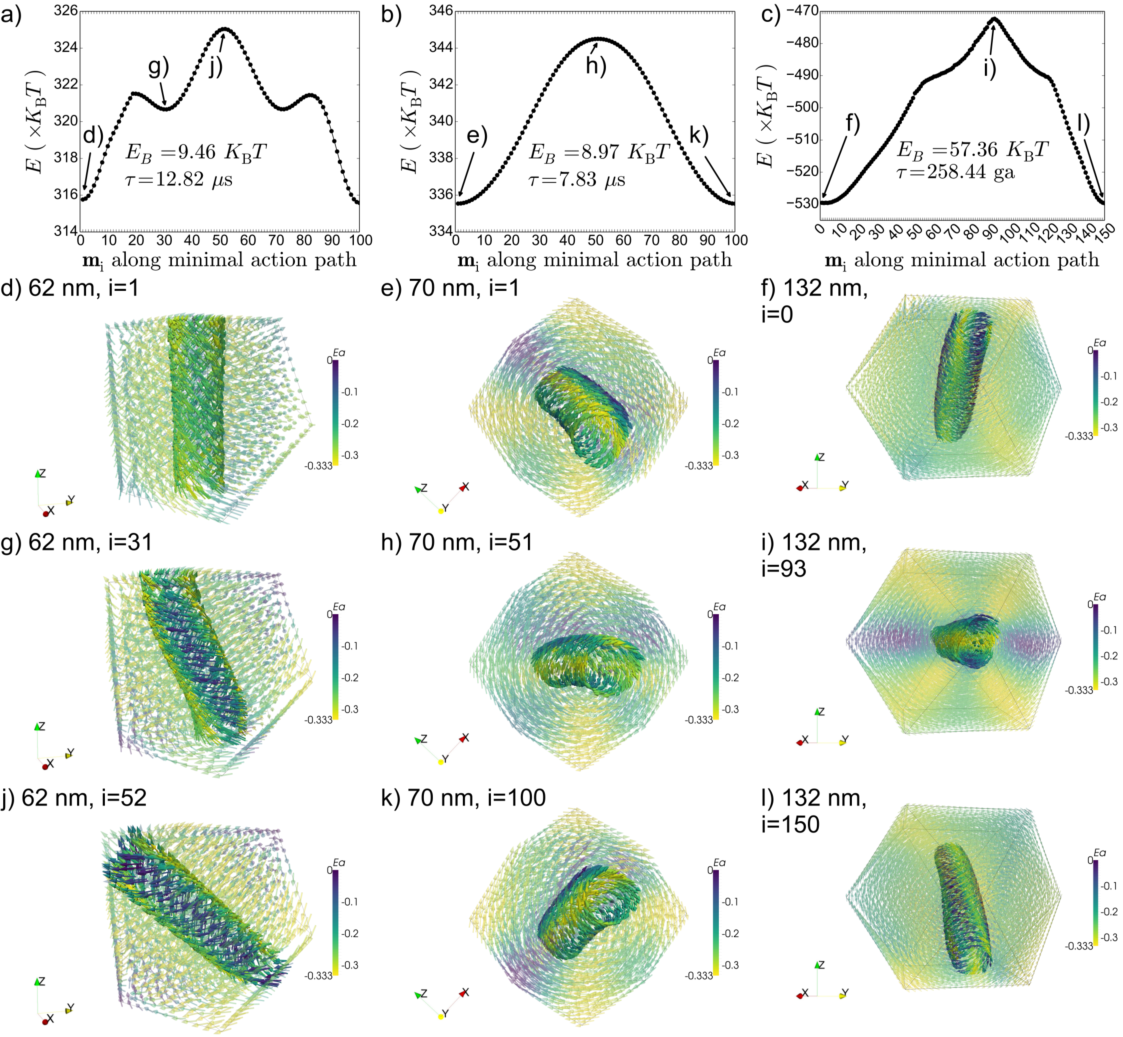
\includegraphics[width=0.8\textwidth]{Chapter_01_Figure_08.pdf}
                  \end{figure}
                \end{frame}

                \begin{frame}
                  \frametitle{Blocking volumes}
                  \begin{figure}[htb]
                    \centering
                    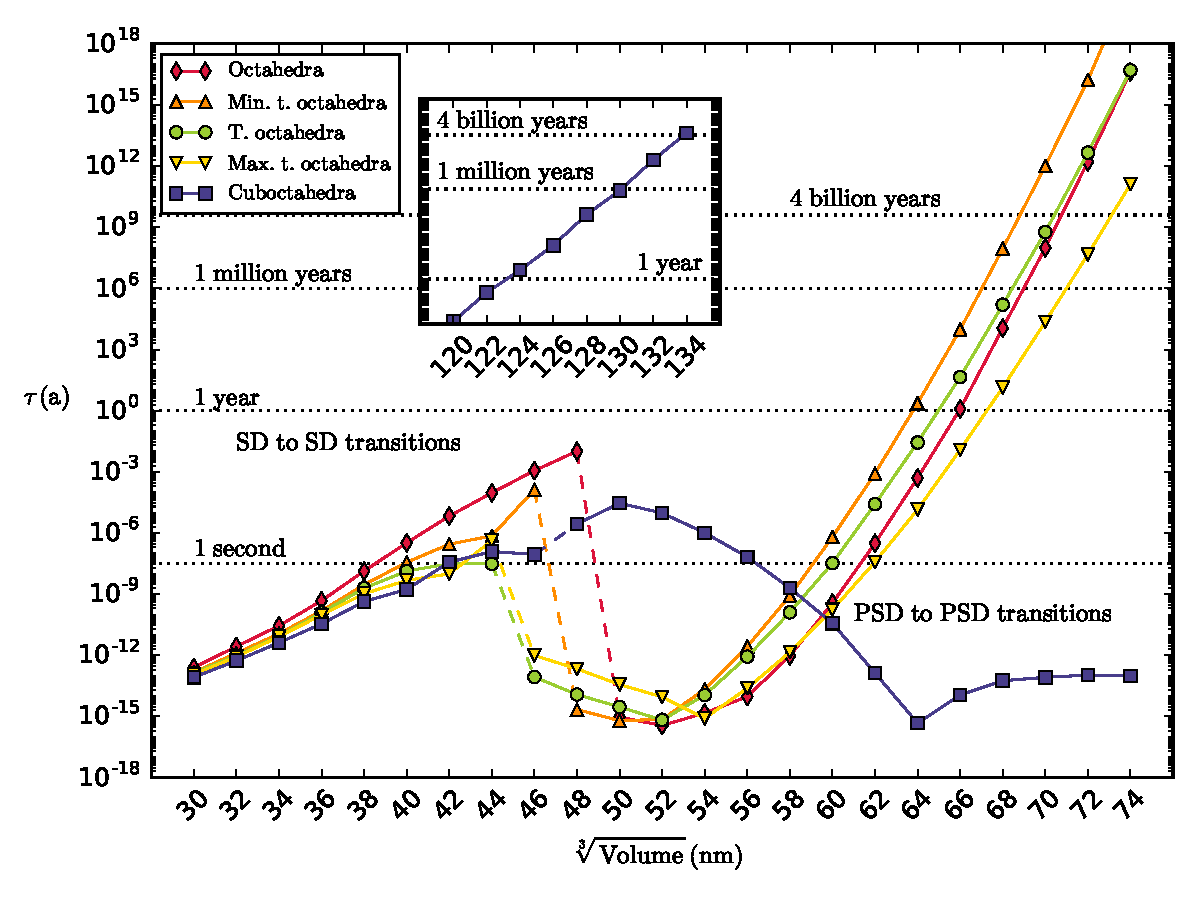
\includegraphics[width=0.9\textwidth]{Chapter_01_Figure_09.pdf}
                  \end{figure}
                \end{frame}

%        \begin{frame}
%          \frametitle{Chapter 1 conclusions}
%          \begin{itemize}
%            \item magnetic domain as a function of size and shape
%            \item blocking volumes as a function of shape
%          \end{itemize}
%        \end{frame}

        \section{Research Chapter II}
        \begin{frame}
          \frametitle{Idealised FORC model}
          To simulate bulk lab measurements, I developed an idealised dipole model of magnetic hysteresis
          \begin{itemize}
            \item a spherical particle is modelled as a dipole
            \item the energy and gradients are expressed in spherical coordinates
            \item a gradient descent algorithm finds the energy minimum for a given external field configuration
          \end{itemize}
        \end{frame}

        \begin{frame}
          \frametitle{Idealised FORC model}
          \begin{figure}[htb]
            \centering
            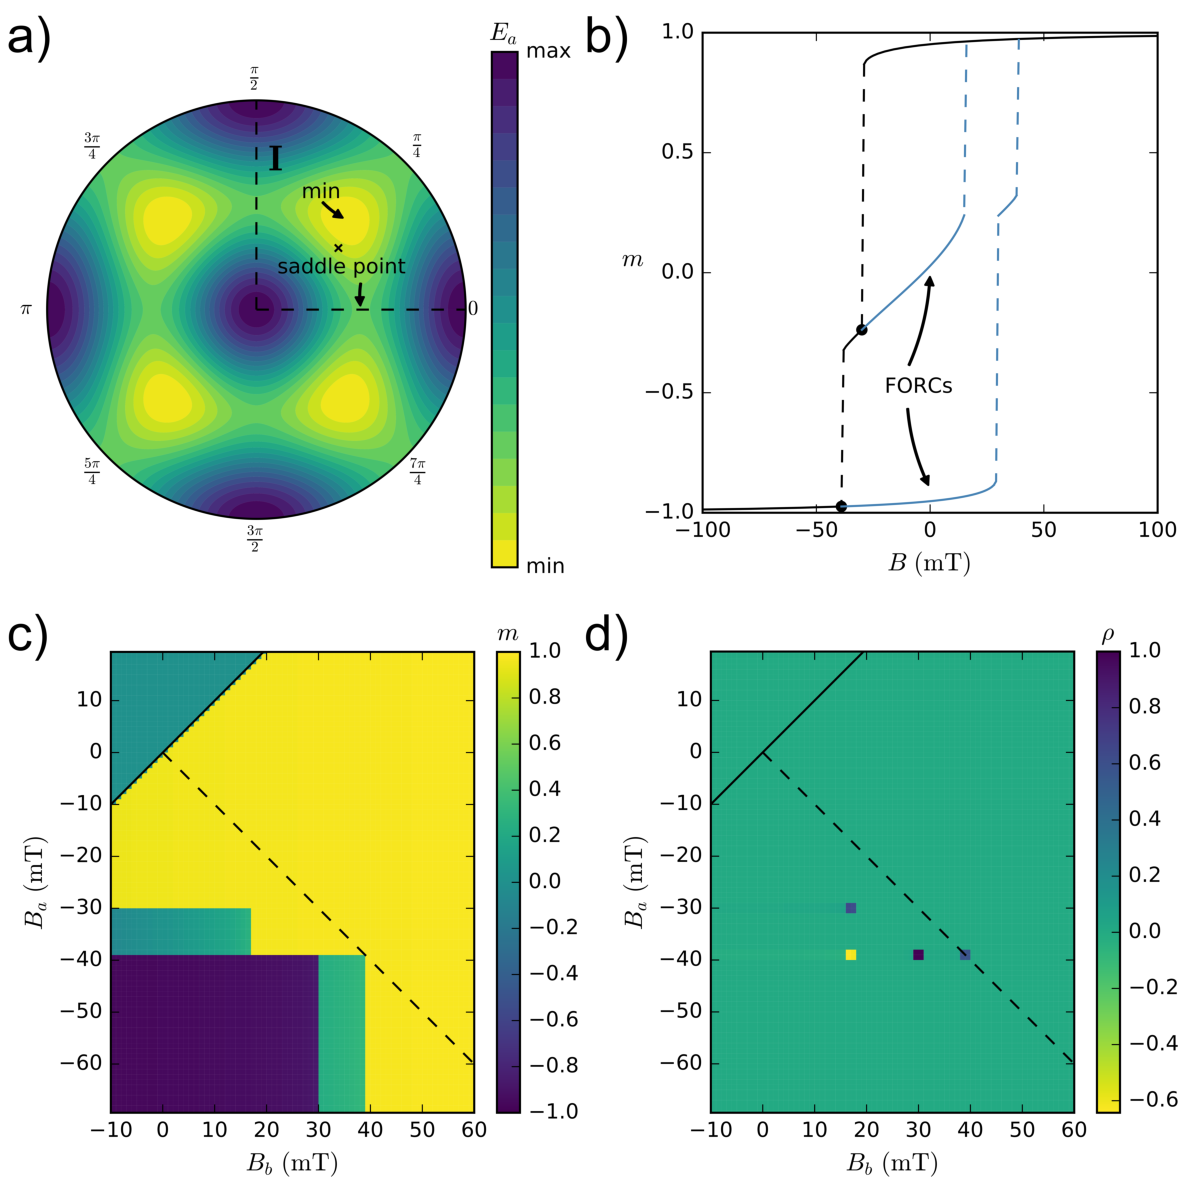
\includegraphics[width=0.7\textwidth]{Chapter_02_Figure_01.pdf}
          \end{figure}
        \end{frame}

        \begin{frame}
          \frametitle{Idealised FORC model}
          \Large The FORC distribution is defined as:\\
          \vspace{2mm} \center $\rho = \rho(\textit{B}_{\textit{b}}, \textit{B}_{\textit{a}}) = -\frac{\text{1}}{\text{2}}\frac{\partial^{\text{2}} \textit{M}}{\partial \textit{B}_{\textit{a}} \partial \textit{B}_{\textit{b}}}$\\
          \vspace{2mm} \flushleft \large The FORC response of a dilute ensemble of randomly aligned particles
          \begin{itemize}
            \item particle orientations uniform over the sphere
            \item no interactions between particles
          \end{itemize}
          \vspace{2mm} \center $\textit{M}(\textit{B}_{\textit{b}}, \textit{B}_{\textit{a}})_{\text{total}} = {\int^{\text{2}\pi}_{\text{0}}}{\int^{\text{2}\pi}_{\text{0}}} \textit{m}(\textit{B}_{\textit{b}}, \textit{B}_{\textit{a}}, \theta, \phi)\,\,\text{sin}\,\theta\,\text{d}\theta\,\text{d}\phi$
        \end{frame}

        \begin{frame}
          \frametitle{Idealised FORC model}
          \begin{figure}[htb]
            \centering
            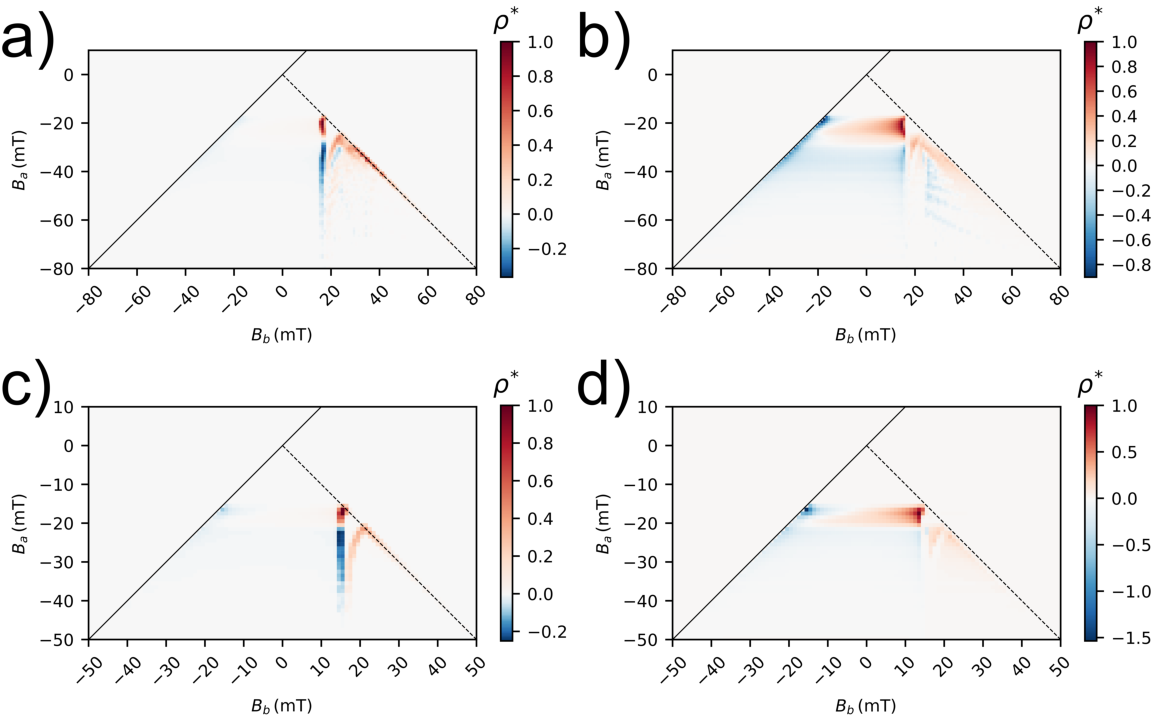
\includegraphics[width=\textwidth]{Chapter_02_Figure_03.pdf}
          \end{figure}
        \end{frame}

        \begin{frame}
          \frametitle{Idealised FORC model}
          \begin{figure}[htb]
            \centering
            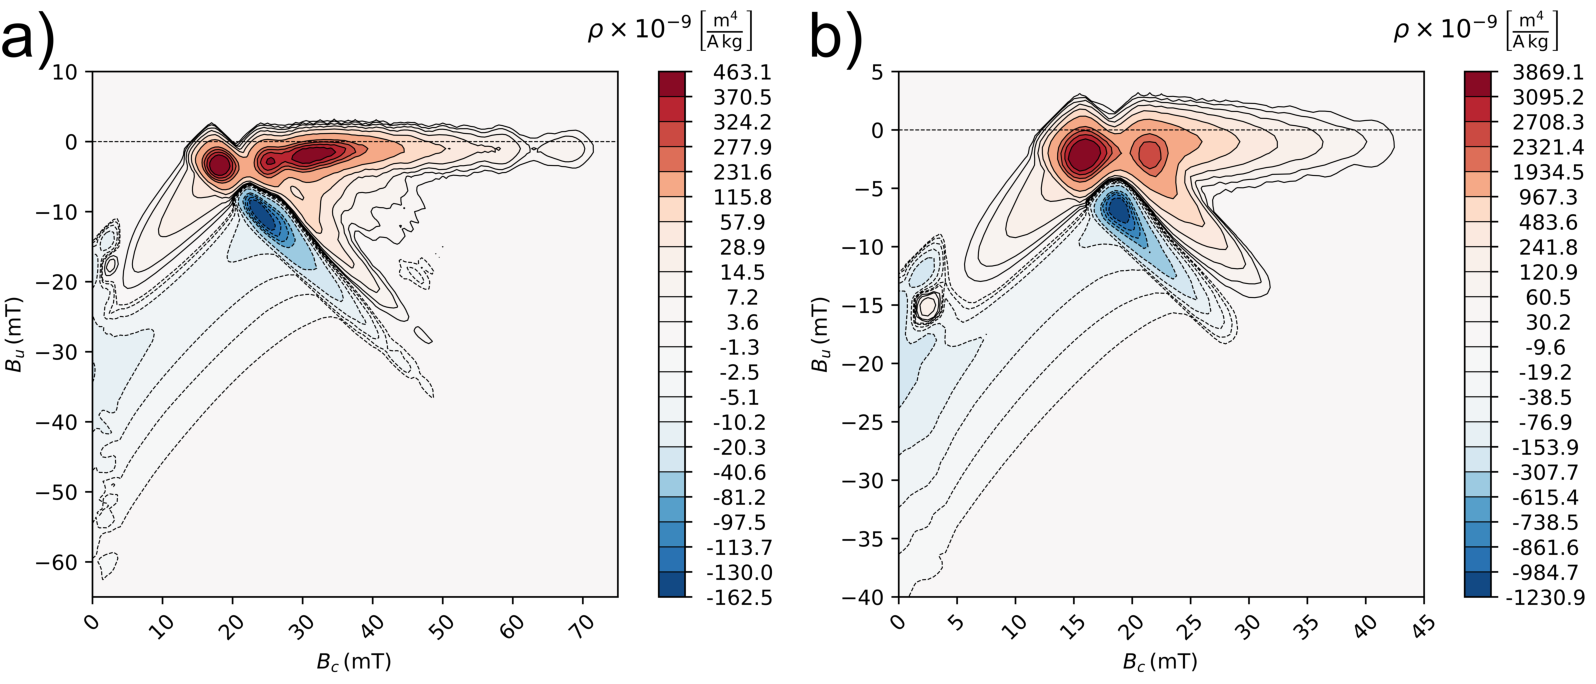
\includegraphics[width=\textwidth]{Chapter_02_Figure_04.pdf}
          \end{figure}
        \end{frame}

        \section{Research Chapter III}
        \begin{frame}
          \frametitle{Micromagnetic FORC model}
          To account for shape and nonuniform magnetisations effects on FORC diagrams, a micromagnetic FEM was employed
          \begin{itemize}
            \item truncated octahedral particles 30 nm to 80 nm
            \item noninteracting particles
            \item micromagnetic model solves for each $m(B_b, B_a)$
            \item to avoid high density of grid points near poles, random orientations used
          \end{itemize}
          \vspace{2mm} \center \Large $\textit{M}(\textit{B}_{\textit{b}}, \textit{B}_{\textit{a}})_{\text{total}} = \frac{\sum_{\textit{i}}^{\textit{n}}\textit{m}_{\textit{i}}(\textit{B}_{\textit{b}}, \textit{B}_{\textit{a}})}{\textit{n}}$
        \end{frame}

        \begin{frame}
          \frametitle{Micromagnetic FORC model}
          \begin{figure}[htb]
            \centering
            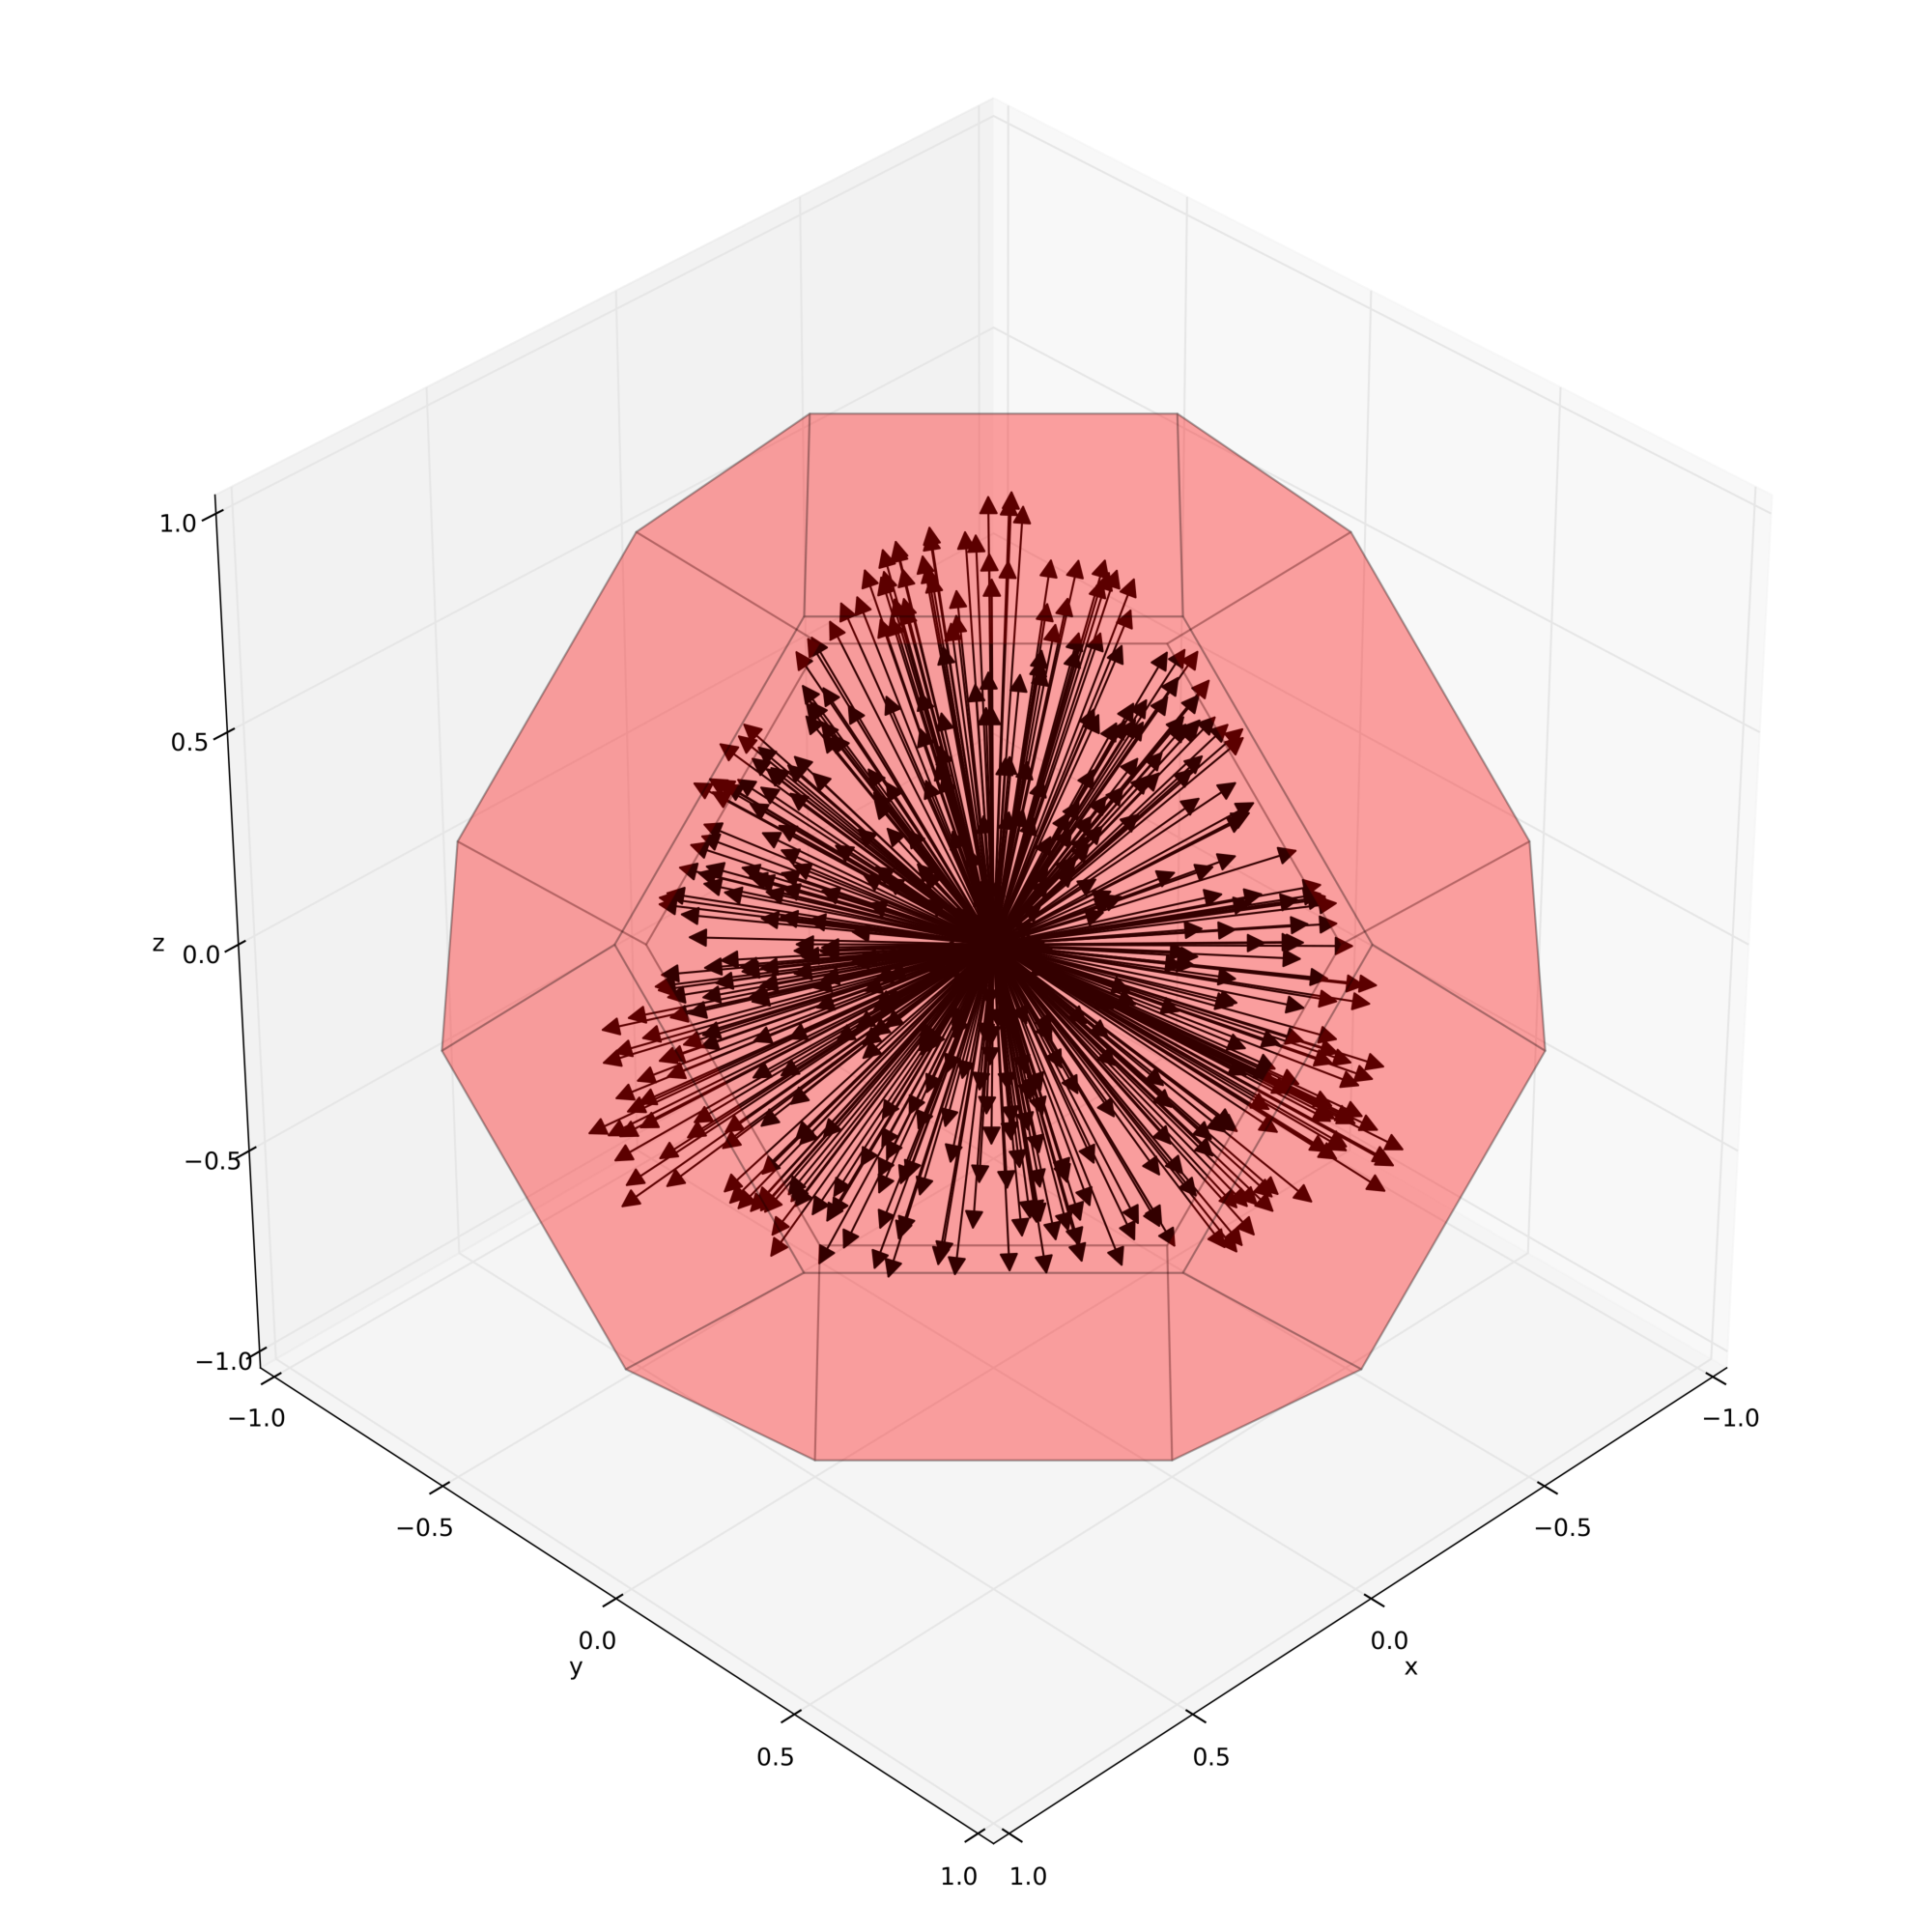
\includegraphics[width=0.7\textwidth]{Chapter_03_Figure_01.pdf}
          \end{figure}
        \end{frame}

        \begin{frame}
          \frametitle{Micromagnetic FORC model}
          \begin{figure}[htb]
            \centering
            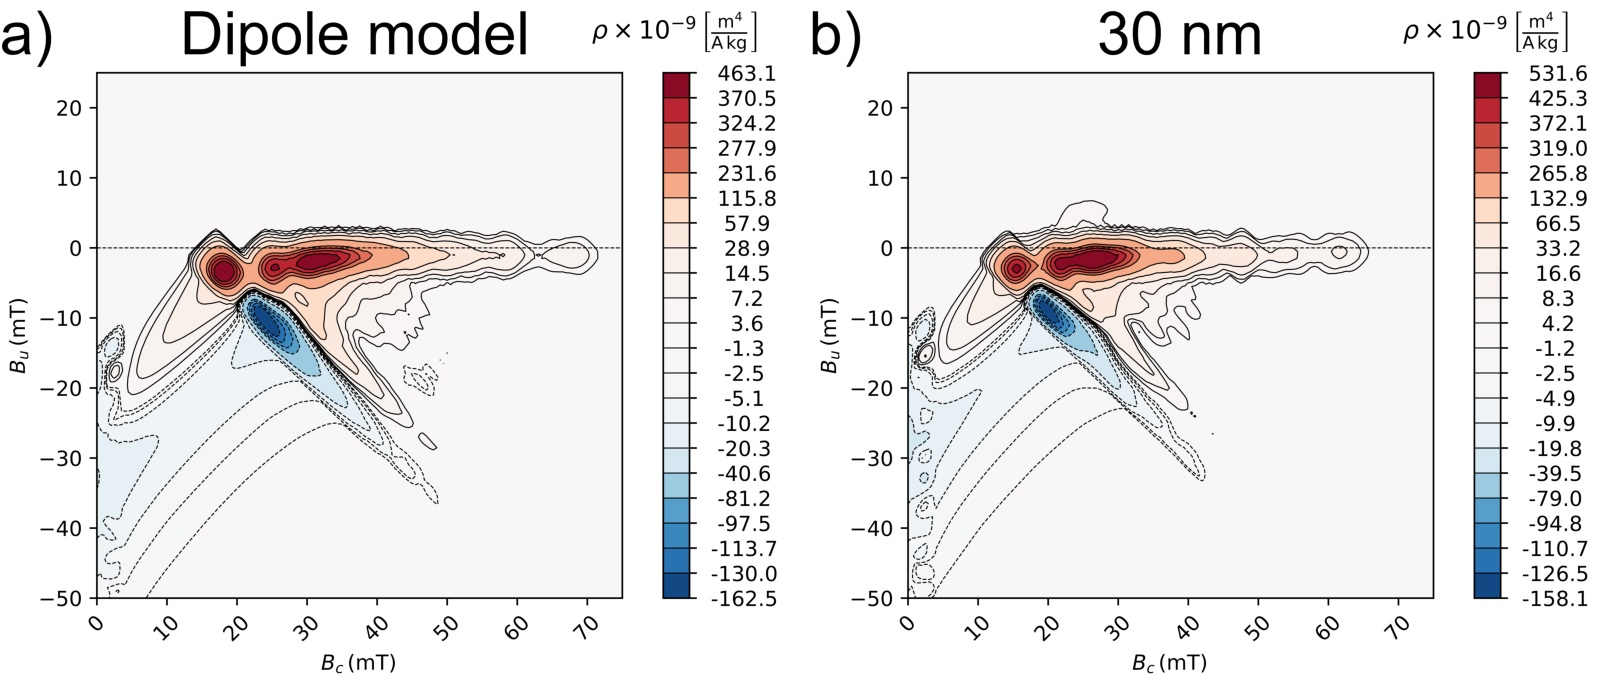
\includegraphics[width=\textwidth]{Chapter_03_Figure_02.pdf}
          \end{figure}
        \end{frame}

        \begin{frame}
          \frametitle{Micromagnetic FORC model}
          \begin{figure}[htb]
            \centering
            \includegraphics[width=0.8\textwidth]{Chapter_03_Figure_03.pdf}
          \end{figure}
        \end{frame}

        \begin{frame}
          \frametitle{Micromagnetic FORC model}
          \begin{figure}[htb]
            \centering
            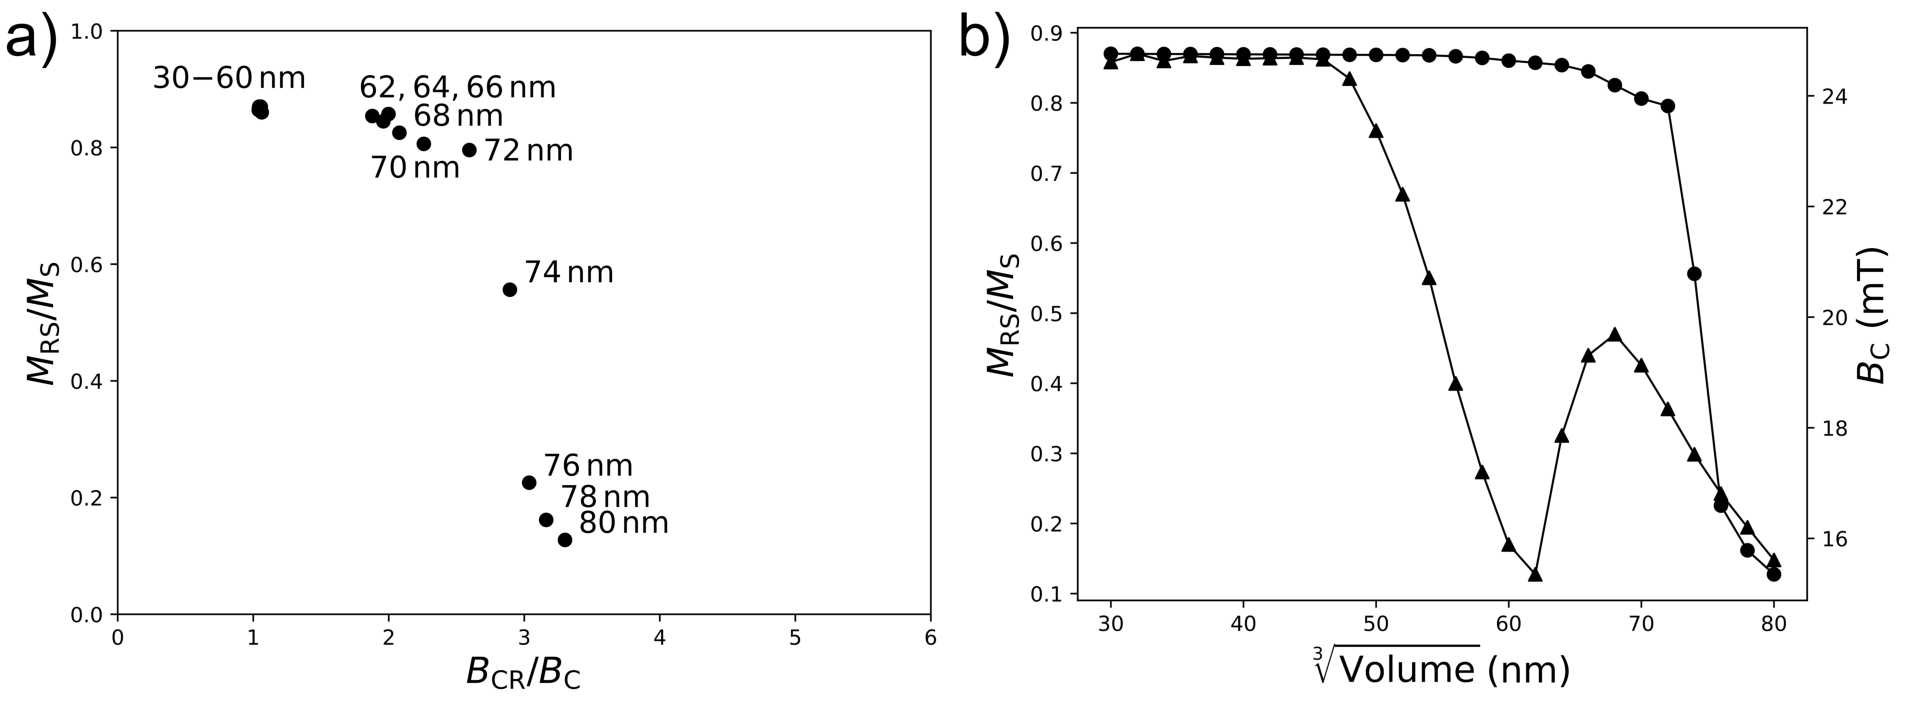
\includegraphics[width=\textwidth]{Chapter_03_Figure_05.pdf}
          \end{figure}
        \end{frame}

        \begin{frame}
          \frametitle{Micromagnetic FORC model}
          \begin{figure}[htb]
            \centering
            \includegraphics[width=0.9\textwidth]{Chapter_03_Figure_09.pdf}
          \end{figure}
        \end{frame}

        \section{Research Chapter IV}
        \begin{frame}
          \frametitle{Framboid FORC model}
          To account for interparticle magnetostatic effects, model framboidal geometries were used to obtain FORC diagrams
          \begin{itemize}
            \item tight clusters of 30 nm truncated octahedral particles
            \item highly interacting particles but no exchange coupling
            \item micromagnetic FEM solves for each $m(B_b, B_a)$
            \item to further reduce computation times, field orientations from an unstructured mesh over the sphere were used
          \end{itemize}
          \vspace{2mm} \center \Large $\textit{M}(\textit{B}_{\textit{b}}, \textit{B}_{\textit{a}})_{\text{total}} = \frac{\sum_{\textit{i}}^{\text{cells}}\textit{m}_{\textit{i}}(\textit{B}_{\textit{b}}, \textit{B}_{\textit{a}}) \textit{A}_{\textit{i}}}{\sum_{\textit{i}}^{\text{cells}}\textit{A}_{\textit{i}}}$
        \end{frame}

        \begin{frame}
          \frametitle{Framboid FORC model}
          \begin{figure}[htb]
            \centering
            \includegraphics[width=0.7\textwidth]{Chapter_04_Figure_01.pdf}
          \end{figure}
        \end{frame}

        \begin{frame}
          \frametitle{Framboid FORC model}
          \begin{figure}[htb]
            \centering
            \includegraphics[width=0.9\textwidth]{Chapter_04_Figure_02.pdf}
          \end{figure}
        \end{frame}

        \begin{frame}
          \frametitle{Framboid FORC model}
          \begin{figure}[htb]
            \centering
            \includegraphics[width=\textwidth]{Chapter_04_Figure_03.pdf}
          \end{figure}
        \end{frame}

        \begin{frame}
          \frametitle{Framboid FORC model}
          \begin{figure}[htb]
            \centering
            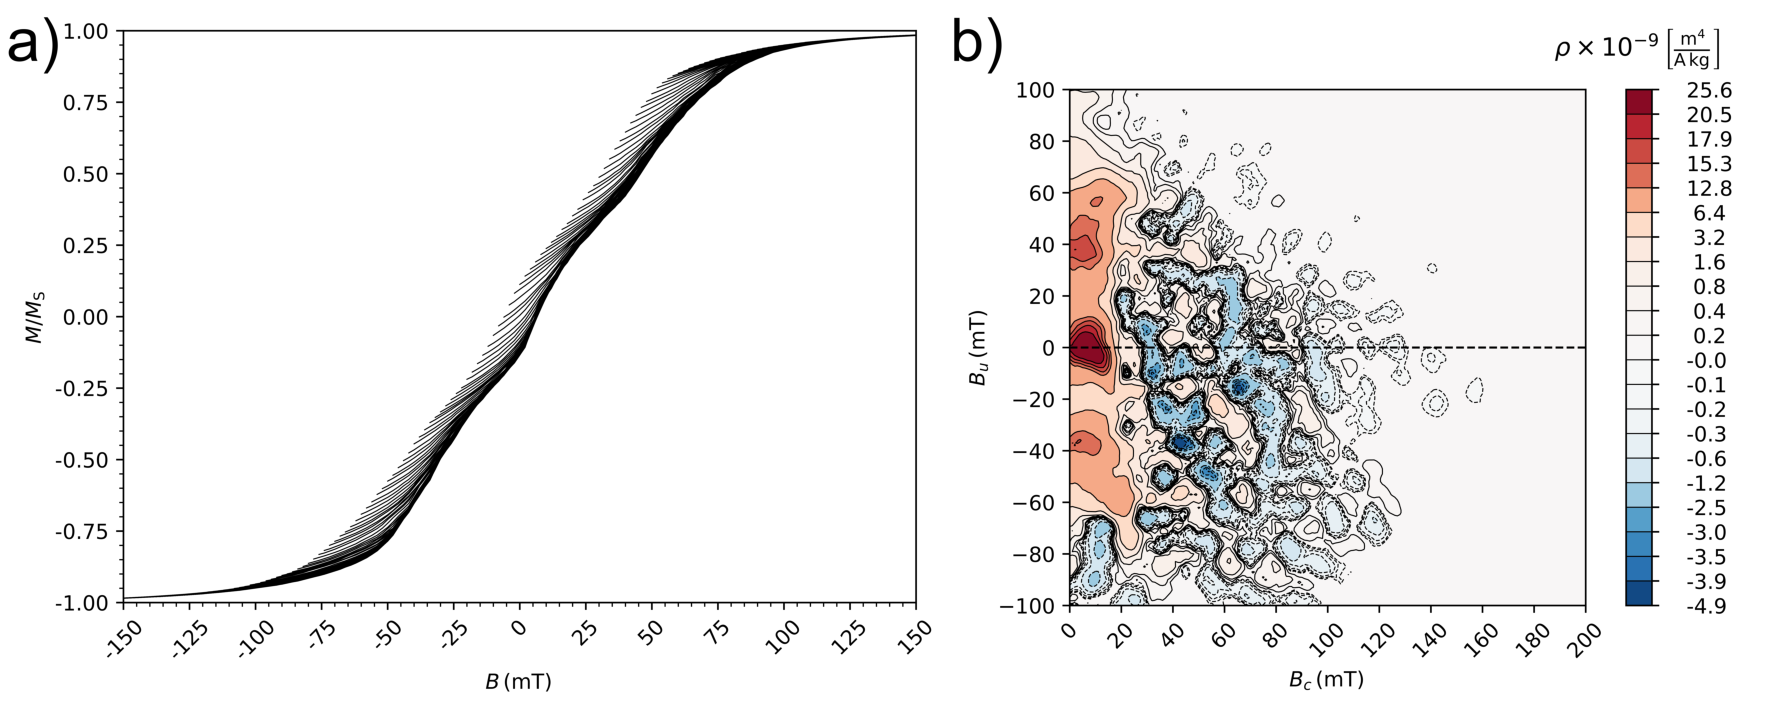
\includegraphics[width=\textwidth]{Chapter_04_Figure_04.pdf}
          \end{figure}
        \end{frame}

        \begin{frame}
          \frametitle{Framboid FORC model}
          \begin{figure}[htb]
            \centering
            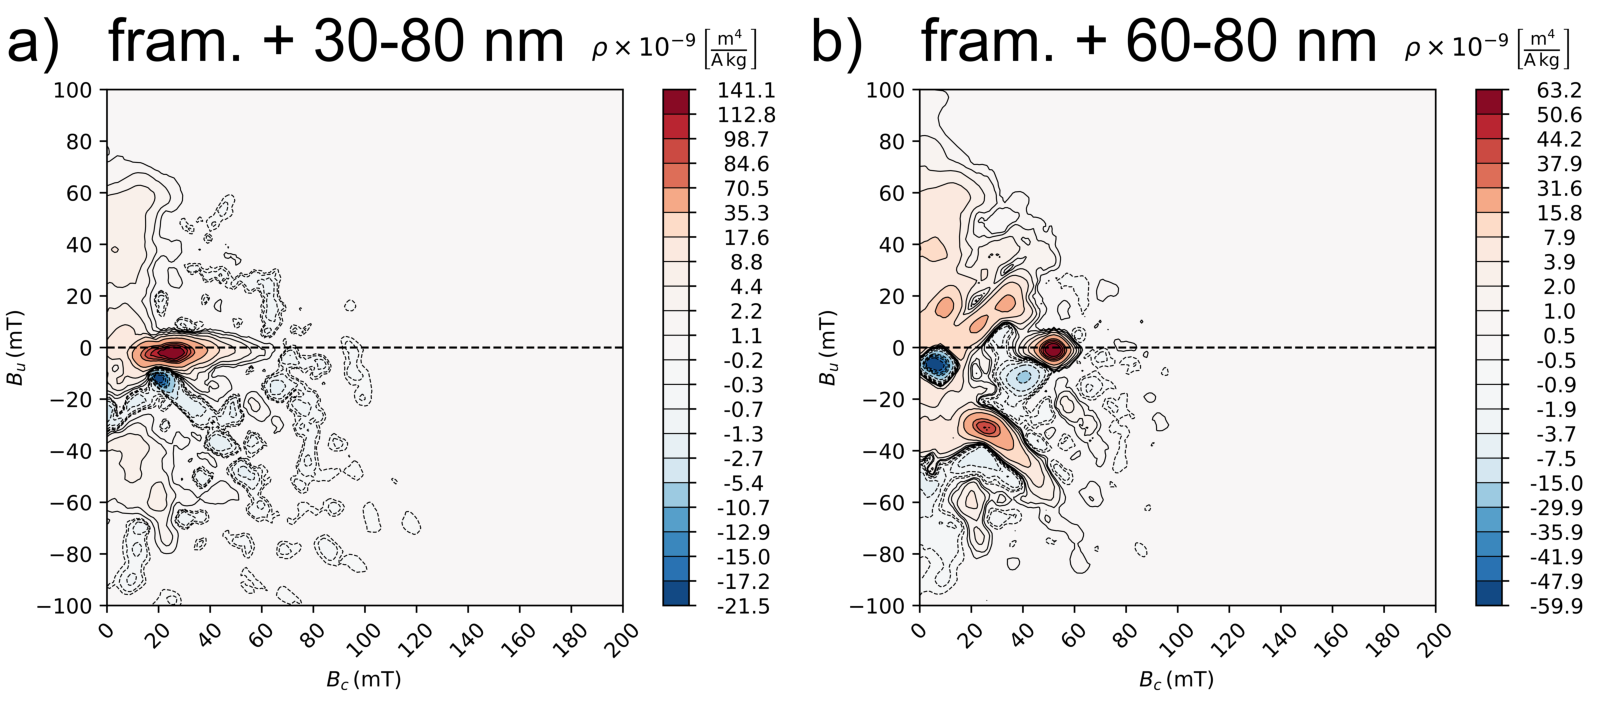
\includegraphics[width=\textwidth]{Chapter_04_Figure_05.pdf}
          \end{figure}
        \end{frame}

        \begin{frame}
          \frametitle{Framboid FORC model}
          \begin{figure}[htb]
            \centering
            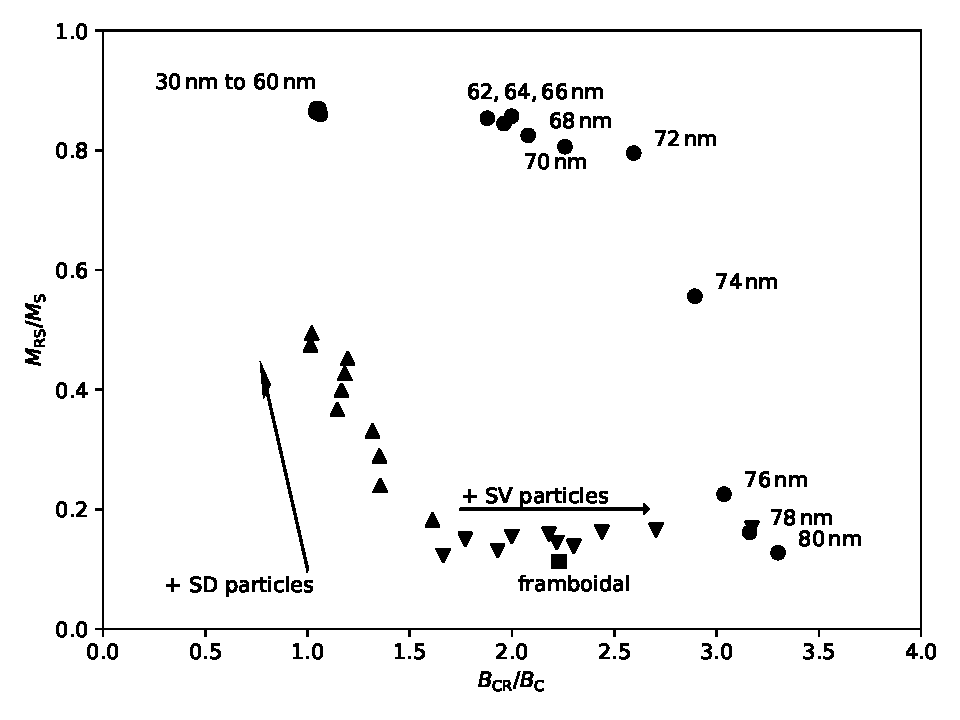
\includegraphics[width=0.9\textwidth]{Chapter_04_Figure_06.pdf}
          \end{figure}
        \end{frame}

        \begin{frame}
          \frametitle{Framboid FORC model}
          \begin{figure}[htb]
            \centering
            \includegraphics[width=0.9\textwidth]{Chapter_04_Figure_07.pdf}
          \end{figure}
        \end{frame}


	\section{Conclusion}
		\begin{frame}
			\frametitle{Conclusions}
			\begin{itemize}
                          \item SD-SV threshold \alert{50 nm}
                          \item SV gradually to MD \alert{$\geq$300 nm}
                          \item Equidimensional \alert{SD greigite essentially SP}
                          \item Palaeomagnetic recorder essentially \alert{SV grains $\geq$70 nm}
                          \item Equidimensional greigite \alert{highly shape-dependent}
			  \item SV transitions through \alert{well-defined states}
                          \item MD transition is continuous from SV nucleation
			\end{itemize}
		\end{frame}

		\begin{frame}
			\frametitle{Conclusions}
			\begin{itemize}
                          \item Noninteracting SD cubic anisotropy particles have \alert{unique FORC patterns}
                          \item SV FORC pattern is more \alert{fragmented}
                          \item SV FORC peaks due to \alert{nucleation and annihilation} of vortices
                          \item SV behaviour for \alert{grains $\geq$70 nm}
                          \item Framboids show \alert{MD-like FORC patterns} even for small particles
			  \item MD-like signals in greigite-rich samples due to \alert{interactions} more than domain state
			\end{itemize}
		\end{frame}

%		\begin{frame}
%			\frametitle{Future work}
%			\begin{itemize}
%                          \item Similar work to Chapter 1 that accounts for elongated grains
%                          \item Estimation of blocking temperatures
%                          \item Interactions
%                          \item \alert{Behaviour in hysteresis/FORCs measurements}
%                        \end{itemize}
%                        \color{ImperialNavy}\huge{and from the experimentalists}
%                        \begin{itemize}
%                          \item \alert{Big challenge:} grow a massive greigite single crystal
%                          \item Constrain \textit{A}, $\textit{K}_{\text{1}}$
%			  \item Measurements at higher temperatures
%                          \item Curie temperature determination
%                          \item Verwey transition?
%			\end{itemize}
%		\end{frame}

\end{document}
